\graphicspath{{./2-Arquitectura/capitulo3/}}

\Capitulo{Motivación}{

Este capítulo se sumerge en la capa de motivación de la arquitectura empresarial. La capa de motivación aborda los aspectos fundamentales que impulsan el cambio y la evolución dentro de la organización, permitiendo una comprensión más profunda de las aspiraciones, necesidades y restricciones que orientan las decisiones estratégicas.

A lo largo de este capítulo, exploraremos los modelos específicos de la capa de motivación, deteniéndonos en cada uno para examinar su papel crucial en la alineación de los objetivos estratégicos con las operaciones diarias. Desde los \textbf{stakeholders clave} y sus \textbf{drivers} hasta los \textbf{principios organizativos} y los \textbf{objetivos estratégicos}, cada elemento modelado contribuye a la construcción de una narrativa coherente que impulsa el cambio positivo.

Este análisis integral, basado en las mejores prácticas de ADM y la expresividad visual de ArchiMate, busca proporcionar una \textbf{visión holística }de la motivación empresarial. A través de esta exploración detallada, se pretende facilitar una toma de decisiones más informada y estratégica, alineada con los valores fundamentales de la organización y orientada hacia el logro de sus metas a largo plazo. \cite{archimate}


}

%--------------Stakeholder-----------------------
\PuntoDeVista{Stakeholder}{imgs/Modelo 1.pdf}{
    El punto de vista de stakeholder representa a los diferentes interesados del sistema, estos stakeholders tienen sus propios objetivos que representan un concepto de valor el cual debe ser medible y cuantificable con el fin de identificar en cualquier momento si se está trabajando para cumplir lo proyectado.
}{imgs/Caso 1.pdf}{Este caso de stakeholders se centra en mostrar cuál es nuestro plan de negocios con el cual obtendremos beneficios por medio de garantizar una alta satisfacción del cliente al ofrecerle gran personalización y una buena relación entre comodidad y precio. }{0.7}{1}

%--------------Realización de Objetivos-----------------------
\PuntoDeVista{Realización de Objetivo}{imgs/Modelo 2.pdf}{
    El modelo permite ver cómo los objetivos se pueden llegar a cumplir definiéndolos por medio de requerimientos y restricciones del sistema. Adicional a esto, dicho modelo también involucra el concepto de principio, elemento que es motivado por el objetivo y representando como una propiedad del sistema.
}{imgs/Caso 2.pdf}{Este caso se centra en garantizar una experiencia satisfactoria para el cliente al personalizar camisetas, considerando tanto aspectos creativos como logísticos.}{0.7}{0.9}

%--------------Contribución de Objetivos-----------------------
\PuntoDeVista{Contribución de Objetivos}{imgs/Modelo 3.pdf}{
    Esta perspectiva utiliza objetivos, principios, requerimientos y restricciones, pero posee un elemento adicional y diferenciador a los demás el cual es llamado influencia. Este elemento permite al analista o diseñador establecer la influencia positiva o negativa que existe entre los objetivos y los requerimientos, proceso que resulta de gran ayuda al momento de analizar el impacto de cada uno de estos e identificar conflictos entre objetivos de los interesados.
}
{imgs/Caso 3.pdf}
{
En este caso se establece que se desea que la satisfacción no solo provenga del objetivo de la personalización de la camiseta, sino de la facilidad de interactuar con la página a la hora, ya sea de pagar o personalizar la camisa.
}{0.9}{0.7}


%--------------Principios-----------------------
\newpage
\section{Principios}
\subsection{Modelo}
\begin{figure}[H]
	\centering	
    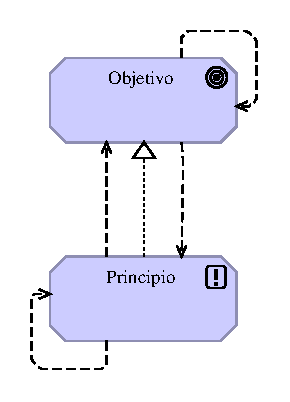
\includegraphics[width=0.3\linewidth]{imgs/Modelo 4.pdf}
	\caption{Modelo Principios}
\end{figure}
 Permite diagramar los principios más relevantes acompañados de sus respectivos objetivos quienes son la fuente de motivación, reflejando en el diagrama aquellos aspectos que son importantes para los interesados y que no se deben olvidar.
\subsection{Caso}
\begin{figure}[H]
	\centering	
    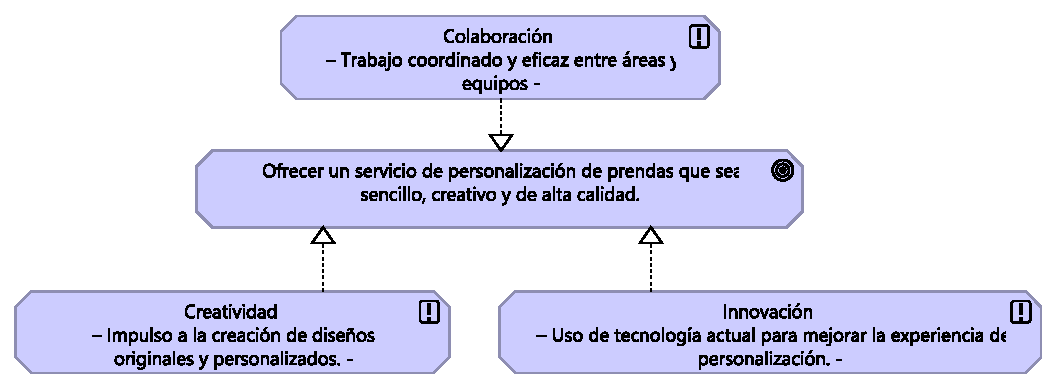
\includegraphics[width=0.9\linewidth]{imgs/Caso 4.pdf}
	\caption{Caso Principios}	
 \end{figure}

La empresa se compromete a una comunicación clara y honesta con sus clientes, ofreciendo diseños originales y de alta calidad, utilizando materiales de primera y tecnología de vanguardia, para garantizar una experiencia personalizada e innovadora en la creación de camisas.
 
%------------Requerimientos-------------------------
\begin{center}
  \begin{minipage}{1\textwidth}
\section{Realización de Requerimientos}

\subsection{Modelo}

\begin{figure}[H]
	\centering	
    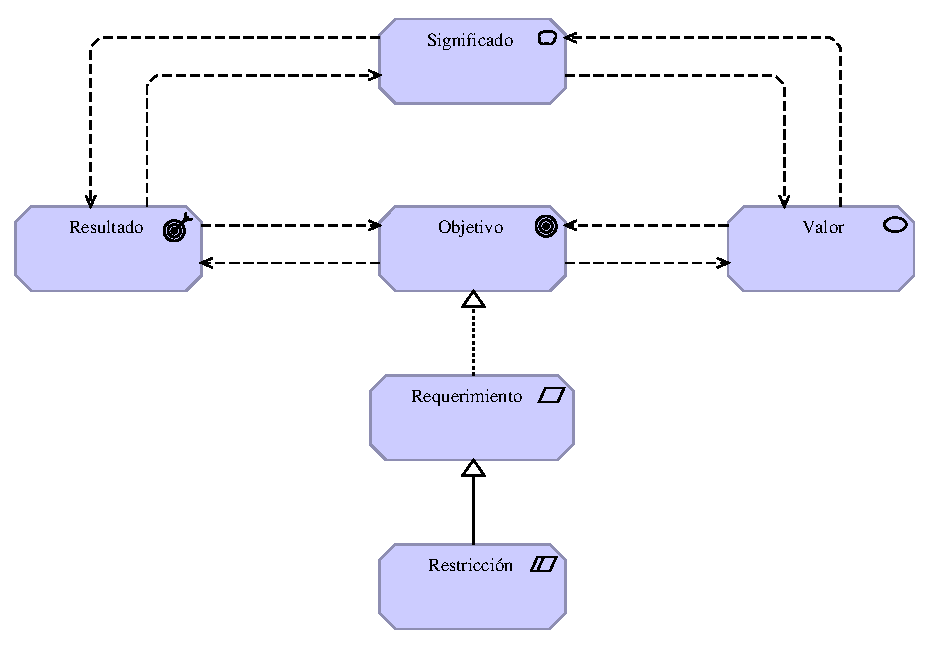
\includegraphics[width=0.9\linewidth]{imgs/Modelo 5.pdf}
	\caption{Modelo Realización de Requerimientos}
\end{figure}


 La perspectiva de realización de requerimientos involucra objetivos que son la base para su elaboración es decir son aquellos que motivan su realización, este diagrama permite modelarlos y establecer un nivel de detalle más avanzado que permitirá identificar elementos adicionales que se representan como especializaciones 
 que en un principio puede que no se hayan detectado.

\end{minipage}
\end{center}
\begin{center}
  \begin{minipage}{1\textwidth}
\subsection{Caso}
\begin{figure}[H]
	\centering	
    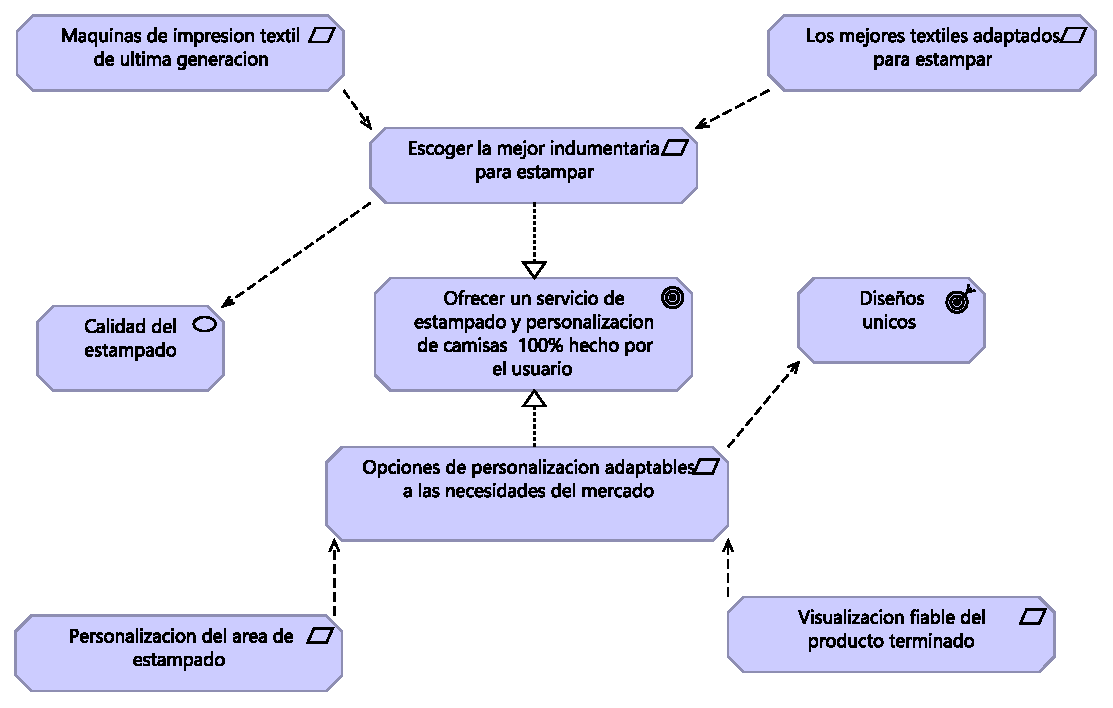
\includegraphics[width=1\linewidth]{imgs/Caso 5.pdf}
	\caption{Caso Realización de Requerimientos}	
 \end{figure}

Para este caso podemos observar a detalle el objetivo que tendrán los requerimientos, enfocados en dos factores clave, los cuales están basados en los principios de calidad e innovación de la empresa.

\end{minipage}
\end{center}

%----------------------Motivacional----------------------



\begin{center}
  \begin{minipage}{1\textwidth}
\section{Motivación}

\subsection{Modelo}

\begin{figure}[H]
	\centering	
    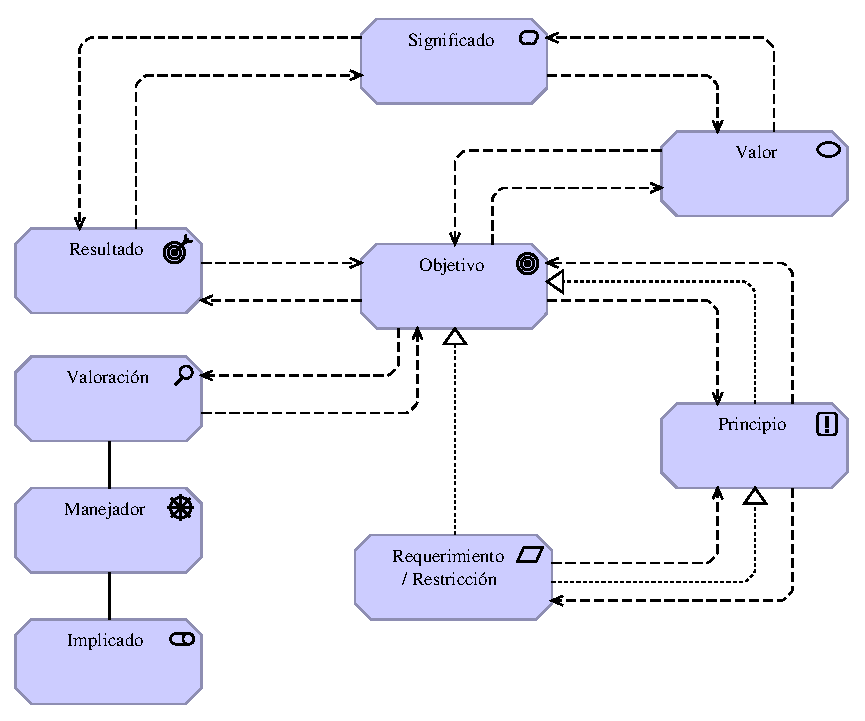
\includegraphics[width=0.9\linewidth]{imgs/Modelo 6.pdf}
	\caption{Modelo Motivación}
\end{figure}


Este punto de vista permite mostrar los principales elementos motivacionales para el desarrollo del sistema, estos se generan mediante los objetivos de cada uno de los participantes y que al final son traducidos en requerimientos que se deben cumplir para satisfacer las necesidades manifestadas.



\end{minipage}
\end{center}
\begin{center}
  \begin{minipage}{1\textwidth}
\subsection{Caso}
\begin{figure}[H]
	\centering	
    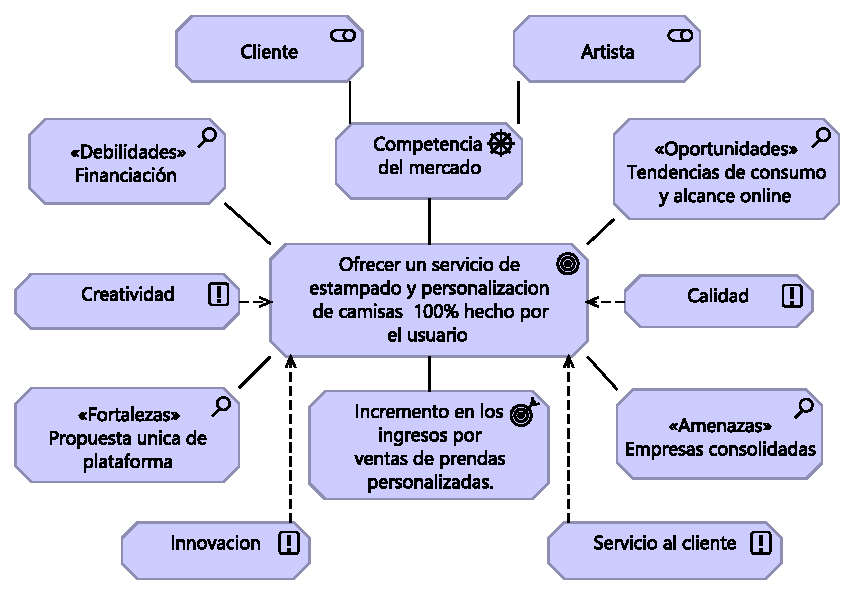
\includegraphics[width=1.1\linewidth]{imgs/Caso 6.pdf}
	\caption{Caso Motivación}	
 \end{figure}

Desde el punto de vista de motivación nos enfocamos en la evaluación de dos características principales, las cuales son la creatividad y la calidad, de las que se realiza el análisis de nuestras debilidades, fortalezas, amenazas y oportunidades. Enfocados en la empresa y los stakeholders principales los cuales son los compradores y artistas.

\end{minipage}
\end{center}